\documentclass[a4paper, ngerman]{article}
\usepackage[ngerman]{babel}
\usepackage[utf8]{inputenc}
\usepackage{fancyhdr}
\usepackage{a4wide}
\usepackage{framed}
\usepackage{lastpage}
\usepackage{graphicx}
\usepackage{float}

\pagestyle{fancy}
\fancyhf{}

\rhead{Kapeller}
\lhead{Wirtschaft Zusammenfassung}
\rfoot{Seite \thepage\ von \pageref{LastPage}}

\renewcommand{\headrulewidth}{1pt}
\renewcommand{\familydefault}{\sfdefault}

\begin{document}

\begin{framed}

    \begin{center}
        \textbf{Wirtschaft | 4AHITN | 2021/22} \\
        MÜ 23.02.2022 \\
        Buch Seiten 176-198
    \end{center}

\end{framed}

\section{Einnahmen-Ausgaben-Rechnung}
\subsection{Abschreibung und Anlagenverzeichnis}
\subsubsection{Abschreibung}
Für \textbf{Anlagegüter}, die \textbf{längerfristig} zur Verfügung stehen, unterliegen durch Gebrauch einer \textbf{Wertminderung}.
\\ \\
Um die Wertminderung mit zu berücksichtigen, dürfen die Anschaffungskosten\footnote{bzw. Herstellungskosten} von Anlagegütern als \textbf{Betriebsausgabe} gültig gemacht werden.
\textbf{ABER} nicht sofort in gesamter Höhe, \textbf{SONDERN} über die Nutzungsdauer verteilt (=abgeschrieben).
\\ \\
\textbf{Geringwertige Wirtschaftsgüter} (Anschaffungswert$<=$800€ netto): können sofort in voller Höhe absetzt werden.
\\ \\
$$
    Abschreibungsbetrag = \frac{Anschaffungskosten}{Nutzungsdauer}
$$
\\ \\
\textbf{Zeitpunkt der Inbetriebnahme}:
\begin{itemize}
    \item 1. Jahreshälfte: gesamter Abschreibungsbetrag darf geltend gemacht werden
    \item 2. Jahreshälfte: halber  Abschreibungsbetrag darf angesetzt werden
\end{itemize}
\textbf{Buchwert}: Wert, der eine Anlage zu einem bestimmten Zeitpunkt hat. Wird aus Anschaffungskosten und bereits vorgenommenen Abschreibung berechnet.
\subsubsection{Anlagenverzeichnis}
... alle Anlagen eines Betriebs
\\ \\
Folgende Angaben:
\begin{itemize}
    \item \textbf{Beschreibung} des Anlagegutes
    \item \textbf{Datum} der Anschaffung und Inbetriebnahme
    \item \textbf{Anschaffungskosten}
    \item Name des \textbf{Lieferanten}
    \item Voraussichtliche \textbf{Nutzungsdauer}
    \item \textbf{Abschreibungsbetrag}
    \item \textbf{Restbuchwert} oder \textbf{Erinnerungswert}\footnote{Wenn Anlage ganz abgeschrieben, wird ein Erinnerungswert (z.B.: 1€) in Anlagenverzeichnis aufgenommen.}
\end{itemize}
\subsection{Sonstige Aufzeichnung - Lohnkonten}
\begin{itemize}
    \item Für jeden \textbf{Arbeitnehmer}
    \item \textbf{Nachweis für Arbeitgeber}, dass Lohnsteuer und Sozialversicherung der Mitarbeiter korrekt ist
    \item \textbf{Bestandteile}
          \begin{itemize}
              \item Name
              \item Versicherungsnummer
              \item Wohnsitz
              \item ...
              \item Pendlerpauschale
              \item Freibetrag laut Finanzamt
              \item Lohn- und Gehaltsabrechnung
              \item ...
          \end{itemize}
\end{itemize}
\subsection{Erfolgsermittlung und Steuererklärung}
Am Jahresende ob, \textbf{Gewinn oder Verlust}.
\subsubsection{Nettomethode}
\textbf{Betriebseinnahmen werden den Ausgaben gegenüber gestellt}. (schnellste Methode)\\ \\
Eigenverbrauch ... Betriebseinnahme \\
Abschreibung ... Betriebsausgabe
\subsubsection{Steuererklärung}
\begin{itemize}
    \item Für \textbf{Abgabenbehörden}
    \item Formular \textbf{E1}
    \item Formular \textbf{E1a}
          \begin{itemize}
              \item die einzelnen Betriebseinnahmen und ausgaben werden bestimmten \textbf{Kennzahlen zugeordnet}
          \end{itemize}
    \item bis um \textbf{30. April des Folgejahres} eingereicht (Finanz-Online bis 30.Juni)
\end{itemize}
\textbf{Verluste} (wenn Ausgaben$>$Einnahmen): kann mit anderen \textbf{positiven Einkünften ausgeglichen} werden. Wenn nicht, dann können sie ins \textbf{Folgejahr vorgetragen} werden
und \textbf{als Sonderausgaben abgezogen} werden.
\\ \\
\textbf{Gewinnfreibetrag}
\begin{itemize}
    \item kann von allen \textbf{natürlichen Personen mit Einkünften aus betrieblicher Tätigkeit} in Anspruch genommen werden
    \item Grundfreibetrag + Gewinnfreibetrag $<=$ 45 350€
    \item maximaler Gewinn: 580 000€
    \item Bestandteile
          \begin{itemize}
              \item Grundfreibetrag
                    \begin{itemize}
                        \item für jeden Unternehmer
                        \item 13\% für Gewinne bis 30 000€ $\rightarrow$ maximal 3 900€
                    \end{itemize}
              \item Investitionsbedingter Gewinnfreibetrag
                    \begin{itemize}
                        \item nur für Unternehmer, die in \textbf{begünstigte Wirtschaftsgüter} investiert haben
                        \item 13\% für Gewinn von 30 000€ bis 175 000€
                        \item 7\% für die nächsten 175 000€
                        \item 4,5\% für die 230 000€
                        \item $\rightarrow$ maximal 45 350€
                    \end{itemize}
          \end{itemize}
\end{itemize}

\section{Doppelte Buchhaltung}
\begin{itemize}
    \item \textbf{Gewinn wird zweifach ermittelt}
          \begin{itemize}
              \item Direkt (GuV-Rechnung)
              \item indirekt (Betriebsvermögensvergleich)
          \end{itemize}
    \item jeder \textbf{Geschäftsfall wird zweifach erfasst}
          \begin{itemize}
              \item zeitlich
              \item systematisch (auf Konten im Hauptbuch)
          \end{itemize}
    \item jeder \textbf{Betrag auf einem Konto}
\end{itemize}
\subsection{Inventur und Inventar}
\begin{itemize}
    \item Welche Vermögensgegenstände sind vorhanden
    \item wer hat diese finanziert
    \item Viel Vermögen $\neq$ "reich sein"
\end{itemize}
\subsubsection{Inventur}
\begin{itemize}
    \item Um \textbf{Auskunft über Vermögen} und Schulden zu bekommen
    \item alle Vermögensgegenstände werden
          \begin{itemize}
              \item gezählt
              \item gemessen
              \item gewogen
              \item bewertet
          \end{itemize}
    \item Ergebnis $\rightarrow$ Inventar
\end{itemize}
\subsection{Bilanz}
\begin{itemize}
    \item \textbf{Gegenüberstellung Vermögen und Schulden}
    \item im Rahmen der \textbf{Jahresabschlussarbeiten}
    \item Zwei Seiten
          \begin{itemize}
              \item Aktiva (oder Soll)
                    \begin{itemize}
                        \item \textbf{Anlagevermögen} +
                        \item \textbf{Umlaufvermögen}
                        \item = Vermögen
                        \item $\rightarrow$ \textbf{Mittelverwendung} (wie werden die Mittel verwendet?)
                    \end{itemize}
              \item Passiva (oder Haben)
                    \begin{itemize}
                        \item \textbf{Eigenkapital} +
                        \item \textbf{Fremdkapital}
                        \item = Kapital
                        \item $\rightarrow$ \textbf{Mittelherkunft} (woher stammen die Mittel?)
                    \end{itemize}
          \end{itemize}
\end{itemize}
\begin{figure}[h]
    \centering
    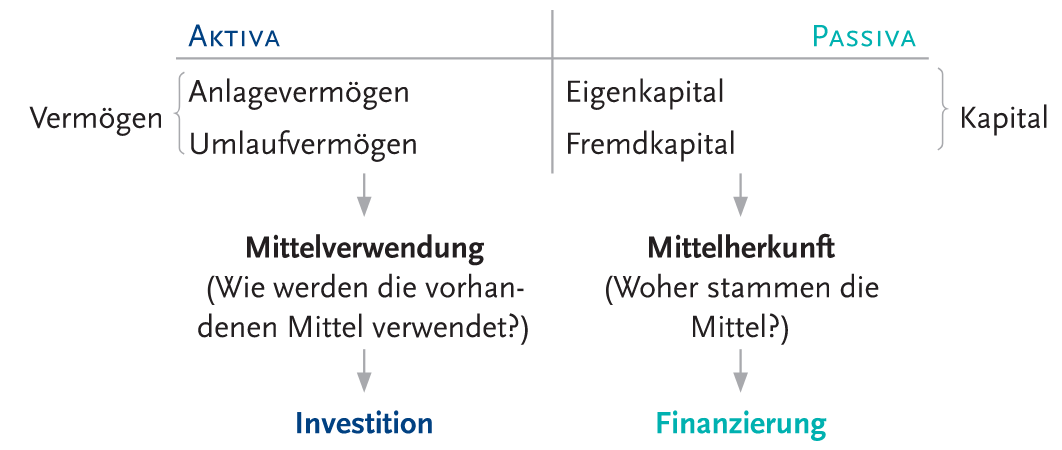
\includegraphics[scale=0.3]{pics/bilanz.png}
    \caption{Bilanz}
\end{figure}

$\rightarrow$ \textbf{Bilanzgleichungen}:
$$
    AKTIVA=PASSIVA
$$
$$
    AKTIVA=EK+FK
$$
$$
    AKTIVA-FK=EK
$$

\noindent \textbf{Anlagevermögen} ... dient Unternehmen längerfristig \\
\textbf{Umlaufvermögen} ... wird laufend verbraucht oder verändert \\
\textbf{Fremdkapital} ... Schulden \\
\textbf{Eigenkapital} ... entscheidende Größe: gibt Auskunft, wie reich ein Unternehmen tatsächlich ist

\subsubsection{Bilanzveränderung}
\begin{itemize}
    \item Jeder Geschäftsfall verändert zwei Positionen der Bilanz
    \item 4 Arten
          \begin{itemize}
              \item Bilanzverlängerung ... Vermehrung des Vermögens durch Vermehrung der Schulden
              \item Aktivtausch ... Ein Vermögensgut wird gemehrt, ein anderes vermindert
              \item Passivtausch ... Schuldenverminderung durch Vermehrung anderer Schulden
              \item Bilanzverkürzung ... Vermögensverminderung durch Schuldenverminderung
          \end{itemize}
\end{itemize}
Dabei wird EK nicht verändert, sondern nur Vermögensteile oder Schulden
$\rightarrow$ Differenz zw. Vermögen und Schulden bleibt gleich
= \textbf{erfolgsneutrale Buchungen}. \\ \\
\noindent
Ändert sich das EK $\rightarrow$ \textbf{erfolgswirksame Buchungen}.
\subsection{Geschäftsfälle auf Konten erfassen}
Jeder Geschäftsfall ändert zwei Positionen der Bilanz $\rightarrow$ zu viel Aufwand für jeden Geschäftsfall neue Bilanz, deshalb
$\rightarrow$ Bilanz am Anfang des Jahres in \textbf{Konten aufteilen}. Am Ende des Jahres werden Konten wieder in Bilanz zusammengefasst.
\subsubsection{Das Konto}
\begin{figure}[h]
    \centering
    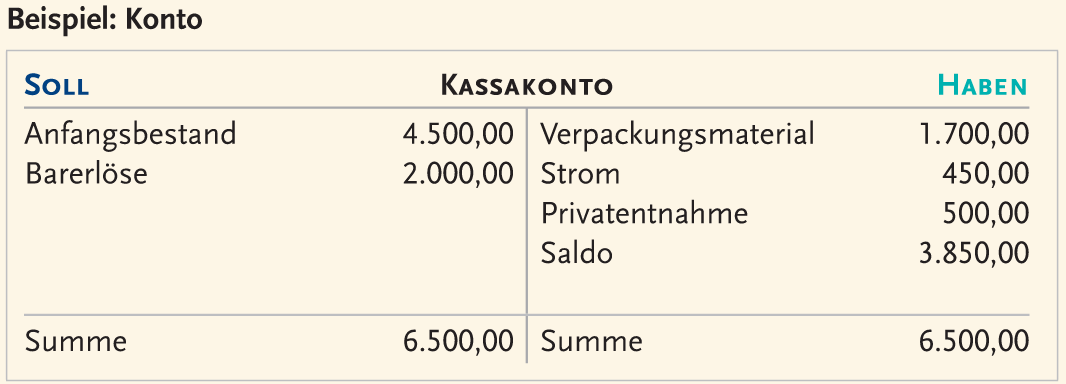
\includegraphics[scale=0.3]{pics/Konto.png}
    \caption{Konto}
\end{figure}

\begin{itemize}
    \item Zwei Seiten
          \begin{itemize}
              \item SOLL (links)
              \item HABEN (rechts)
          \end{itemize}
    \item am Ende des Abrechnungszeitraums wird Endbestand (\textbf{Saldo}) berechnet.
    \item Mithilfe von Bilanz und GuV-Rechnung\footnote{Gewinn-und Verlust-Rechung; Aufwände und Erträge gegenüber gestellt} werden vier verschiedene Arten von Konten abgeleitet:
          \begin{figure}[h]
              \centering
              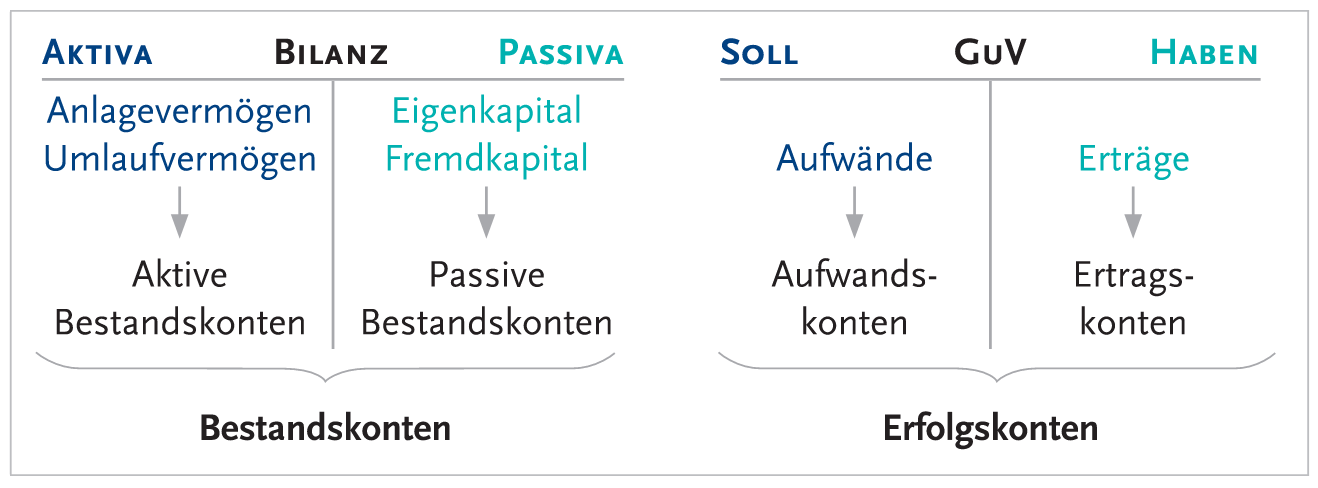
\includegraphics[scale=0.2]{pics/uebersicht_konten.png}
              \caption{Übersicht Konten}
          \end{figure}
          \begin{itemize}
              \item Bestandskonten: beeinflussen \textbf{Vermögens- bzw. Schuldensituation}
                    \begin{itemize}
                        \item \textbf{aktive Bestandskonten}
                              \begin{itemize}
                                  \item \begin{figure}[h]
                                            \centering
                                            
\includegraphics[scale=0.18]{pics/aktiv_bestandkonto.png}
                                            \caption{Aktives Bestandskonto}
                                        \end{figure}
                              \end{itemize}
                        \item \textbf{passive Bestandskonten}:
                              \begin{itemize}
                                  \item \begin{figure}[h]
                                            \centering
                                            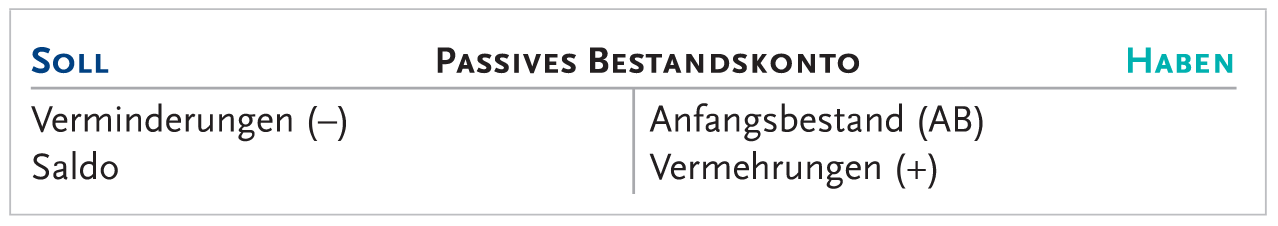
\includegraphics[scale=0.18]{pics/passiv_bestandkonto.png}
                                            \caption{Passives Bestandskonto}
                                        \end{figure}
                              \end{itemize}
                    \end{itemize}
              \item Erfolgskonten: beschäftigen sich mit \textbf{Aufwänden} und \textbf{Erträgen} \\
                    $\rightarrow$ Aufwände vermindern EK, Erträge vermehren EK (\textbf{Gewinn oder Verlust}) \\
                    \textbf{Aufwands- und Ertragskonto} ... Unterkonto von EK \\ \\
                    Aufwand $\rightarrow$ Kapitalverminderung $\rightarrow$ \textbf{SOLL} \\
                    Ertrag $\rightarrow$ Kapitalvermehrung $\rightarrow$ \textbf{HABEN} \\ \\
                    Aufwands- und Ertragskonto $\rightarrow$ GuV-Rechnung $\rightarrow$ Eigenkapital
                    \begin{figure}[h]
                        \centering
                        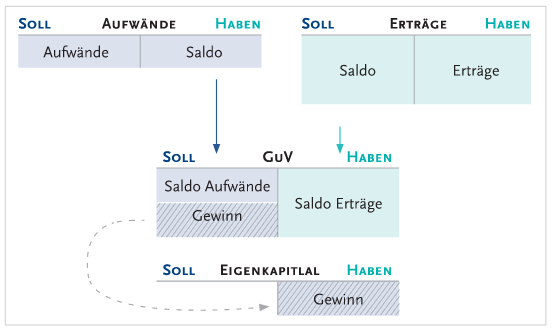
\includegraphics[scale=0.53]{pics/auf_ertrag.png}
                        \caption{Aufwands- und Ertragskonto}
                    \end{figure}
          \end{itemize}
\end{itemize}
\textbf{Gliederung der Konten}
\begin{itemize}
    \item wie viele Konten, hängt ab von
          \begin{itemize}
              \item Größe des Unternehmens
              \item Branche
              \item Anforderungen an Rechnungswesen
          \end{itemize}
    \item Übersicht der Konten: \textbf{Kontenplan}
    \item Kontenklassen:
          \begin{figure}[H]
              \centering
              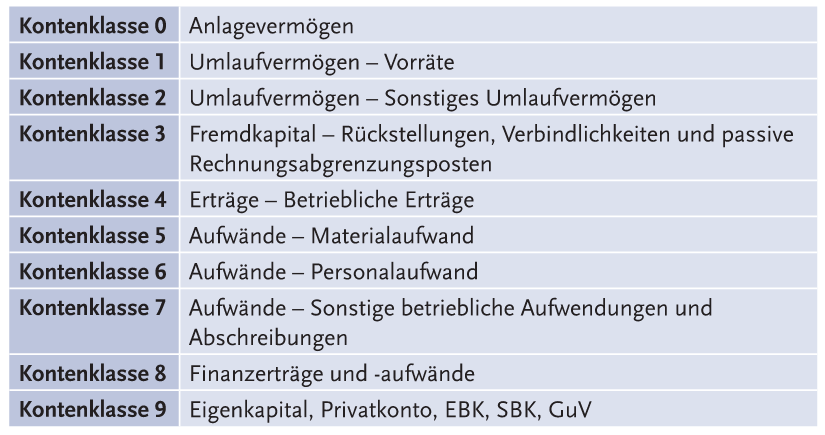
\includegraphics[scale=0.4]{pics/kontenklassen.png}
              \caption{Kontenklassen}
          \end{figure}
\end{itemize}
\subsubsection{Buchen}
Geschäftsfälle werden in verkürzter Form dargestellt \\
keine Buchung ohne Beleg \\
$\rightarrow$ \textbf{Buchungssatz bildet einen Beleg ab} \\ \\

\begin{tabular}{ c c c }
    Mittelverwendung    &             & Mittelherkunft       \\
    FÜR                 &             & VON                  \\
    Konto Soll + Betrag & \textbf{/}  & Konto Haben + Betrag \\
    Konto Soll + Betrag & \textbf{an} & Konto Haben + Betrag
\end{tabular}

\end{document}